%%%%%%%%%%%%%%%%%%%%%%%%%%%%%%%%
\section{Overview}
\label{sec:detectors-fd-ref-ov}


The alternative detector design benefits of 13 years of R\&D activity and two programs funded by the European Union for a total budget of 17 Meur which resulted in the LAGUNA-LBNO design study concluded in August 2014. The LAGUNA-LBNO design study allowed to define, in collaboration with several industrial partners, an optimized configuration for a long baseline experiment  experiment with associated technological developments, innovative solutions and full costing. In particular, since the very beginning, these studies were focused on the underground implementation of a very large liquid argon detector (GLACIER) aiming at optimizing the construction and installation costs and making affordable the detector implementation and operation. This optimization concerned not only the double-phase readout concept but also many technical aspects in the underground design such as the tank, the field cage, the cathode  and the definition of the logistics and the detector assembly sequence. All these technical developments are documented in the deliverable to the EU \cite{LAGUNA-LBNO-deliv}.

Following the GLACIER concept, the double-phase LAr TPC detector has the shape of a vertically standing volume, where electrons are drifted vertically towards the liquid-vapor interface, extracted from the liquid into the gas phase, amplified and collected at a segmented anode \cite{Badertscher:2013wm,Badertscher:2012dq,Badertscher:2010zg}. One of the novel features of the double-phase TPC is the electron amplification in the gas phase. This allows to obtain a robust and tunable signal to noise ratio. Gas amplification in extremely pure argon gas has been obtained using a new Micro Pattern Gas Detector call LEM (Large Electron Multiplier). The detector is configured as a liquid argon TPC with liquid-to-gas ionization electron extraction and multiplication before collection.

The transfer of electrons in excess from a condensed non-polar fluid to its saturated vapor using an electric field is a phenomenon investigated since the seventies~\cite{Dolgoshein1970}. In particular, in argon it is experimentally shown that the electrons are extracted in two stages. Near the triple point part of the charge is emitted on time scales that can be as high as 1~ms, strongly dependent on the electric field applied~\cite{Gushchin1982b, Borghesani1990}, while at larger temperatures the emission takes less than 100~ns. At high electric fields the slow extraction time reduces, and the fraction of the slowly extracted electrons becomes negligible (see Figure~\ref{Fig:extractionVsElectricField}). This behavior can be understood in the framework of the Schottky model of electric field enhanced thermionic emission~\cite{Murphy1956}.For practical purpose the efficiency of the electron extraction saturates for voltage differences above a few kV/cm

In the double-phase LAr TPC, an electric field of the order of 2 kV/cm created by submersed grid at the liquid-gas interface allows for 100\% efficiency extraction of the electrons from the liquid to the gas phase. The ionization charge is then amplified by avalanches occurring in the gas in the micropattern structure of the LEM and collected in a 2-dimensional readout plane on the top of the volume, on readout units, combining both the amplification and collection functions, with an area of $0.5\times 0.5$~m$^2$ and finely segmented with a 3~mm strip pitch. The typical amplification achieved in this configuration is around a few tens and it allows to compensate for the charge losses due to the presence of electronegative impurities along very log drift paths achieving a S/N ratio exceeding 100 for a particle at the ionization minimum (m.i.p.).

The full active volume  is under a drift electric field  $E{\simeq} 0.5-1.0$~kV/cm generated from a bottom cathode plane and kept uniform by a stack of field shaping electrodes, several equally-spaced stainless-steel tubes along a square path with round corners. All this system is held in place by insulating mechanical structures hung from the top cap of the vessel. These electrodes are polarized at linearly decreasing voltage from the cathode voltage to ground. 


\begin{cdrfigure}[The 50kton LBNO detector. ]{LBNO_50}{The 50 kton LBNO detector.}
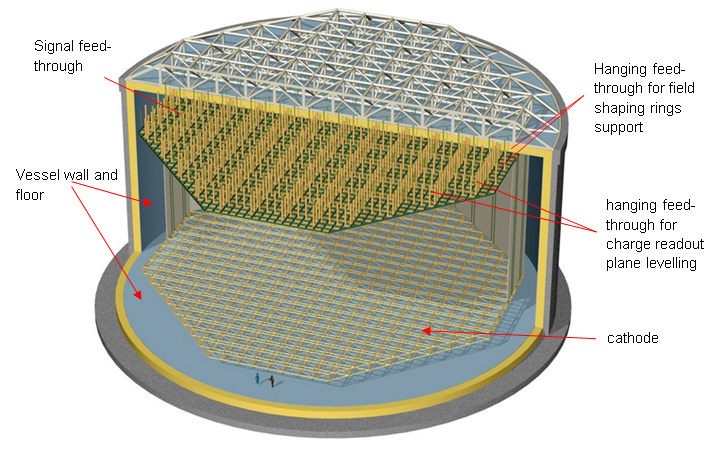
\includegraphics[width=\linewidth]{LBNO50kton2}
\end{cdrfigure}

The anode deck is also independently suspended with stainless-steel ropes linked to the top roof  which allow to adjust its distance and parallelism with respect to the liquid surface.  The bottom field is  closed by a transparent cathode and the top field by an anode, which also  serves as the charge readout: the Charge Readout Plane (CRP).  The cathode plane is gridded and it is transparent to light to allow the detection of the scintillation light by an array of photomultipliers uniformly distributed  at a distance of $1m$  below the cathode and mounted on the tank bottom surface. Ionization charge signals are sent to a set of signal feedthroughs located on the top face of the hosting LAr vessel and hosting the cold readout electronics. Other chimneys/feedthroughs are foreseen for HV, top readout plane suspension and level regulation, PMT high voltage and signal readout, monitoring instrumentation (level, temperatures, strain gauges, etc ...) The front-end electronics is based on analog preamplifiers implemented in CMOS ASIC circuits for high integration and large scale affordable production. The baseline design is to integrate this electronics on the feed-through flange terminating the chimneys on the roof of the tank, under the insulation layer in order to be cooled to a temperature near that of liquid argon.

The double-phase readout scheme, based on the extraction of the electrons to the gas phase and their amplification and collection on the CRP, has been successfully demonstrated on several prototypes  by an R\&D activity which spans over more than 10 years.The design of very large (20 to 50 kton) underground detectors based on this concept has been developed in great detail in the context of the LAGUNA and LAGUNA-LBNO design studies.  The CERN WA105 experiment is intended to show a full scale implementation of this technique, as well as of other technologies developed in the framework of the LAGUNA-LBNO design study for the construction of large underground TPC detectors.  All the key subsystems have been designed taking into account their scalability to a large detector.  In 2018, this demonstrator will be tested and calibrated with a charged particle beam (pion, muons, electrons).

One of the main features of the double phase concept is that it provides inside the TPC field cage a large homogeneous fiducial volume for neutrino interactions, purely constituted by liquid argon and with no passive material. The charge produced in this volume is read out on the top surface in a projective way, with practically no dead regions. The charge is readout in two collection views with no use of induction views, which is also an important asset in the case of complicated topologies. 

Situated in the vapor phase on top of the LAr volume the CRP  provides an adjustable charge gain and two independent readout views, each with a canonical and optimal pitch of 3.125 mm.  With T0 time information provided by the LAr scintillation readout by the PMT array, they provide a real-time three-dimensional (3D) track imaging with dE/dx information. The S/R ratio is increased by at least one order of magnitude by the possibility of amplifying the charges with avalanches in the gas phase.  This significantly improves the event reconstruction quality with a lower energy deposition threshold and a better resolution per volumetric pixel (voxel) compared to a conventional single-phase LAr-TPC. 

The double phase concept is well suited for giant detector size since the increased noise level when going into larger detector size would be compensated by improving the signal amplitude thanks to the charge amplification.  This arrangement simplifies the construction and optimally exploits the possibility of long drifts, limiting the number of read-out channels, increasing the detector size, limiting dead spaces and lowering costs.

\subsection{LAr purity requirements}

As discussed in the previous section, one of the main features of the double phase design is a long drift path. This requires an ultra-high level of purity in the medium, which is however not higher of the one required by the single-phase LAr TPC implementation with a drift path of a few m. 

The expected ionization charge attenuation due to attachment to impurities as a function of the drift path for various oxygen-equivalent impurity levels and electric fields is shown in Figure~\ref{Fig:larimpuritycomp}.

The arrows indicate the drift length of the ICARUS T600~\cite{Amerio:2004ze},  MicroBOONE~\cite{Chen:2007ae}, LBNE~\cite{Akiri:2011dv} 
and LAGUNA-LBNO GLACIER~\cite{Rubbia:2009md,Rubbia:2010zz}.


\begin{cdrfigure}[Charge attenuation as a function of the drift]{larimpuritycomp}{Expected ionisation charge attenuation due to attachment to impurities as a function of the drift path for 0.2~ppb, 20~ppt and  2~ppt Oxygen-equivalent impurity levels and electric fields in the range 0.5--1.5~kV/cm. The arrows indicate the drift length of the ICARUS T600, MicroBOONE, LBNE and LAGUNA-LBNO GLACIER.}
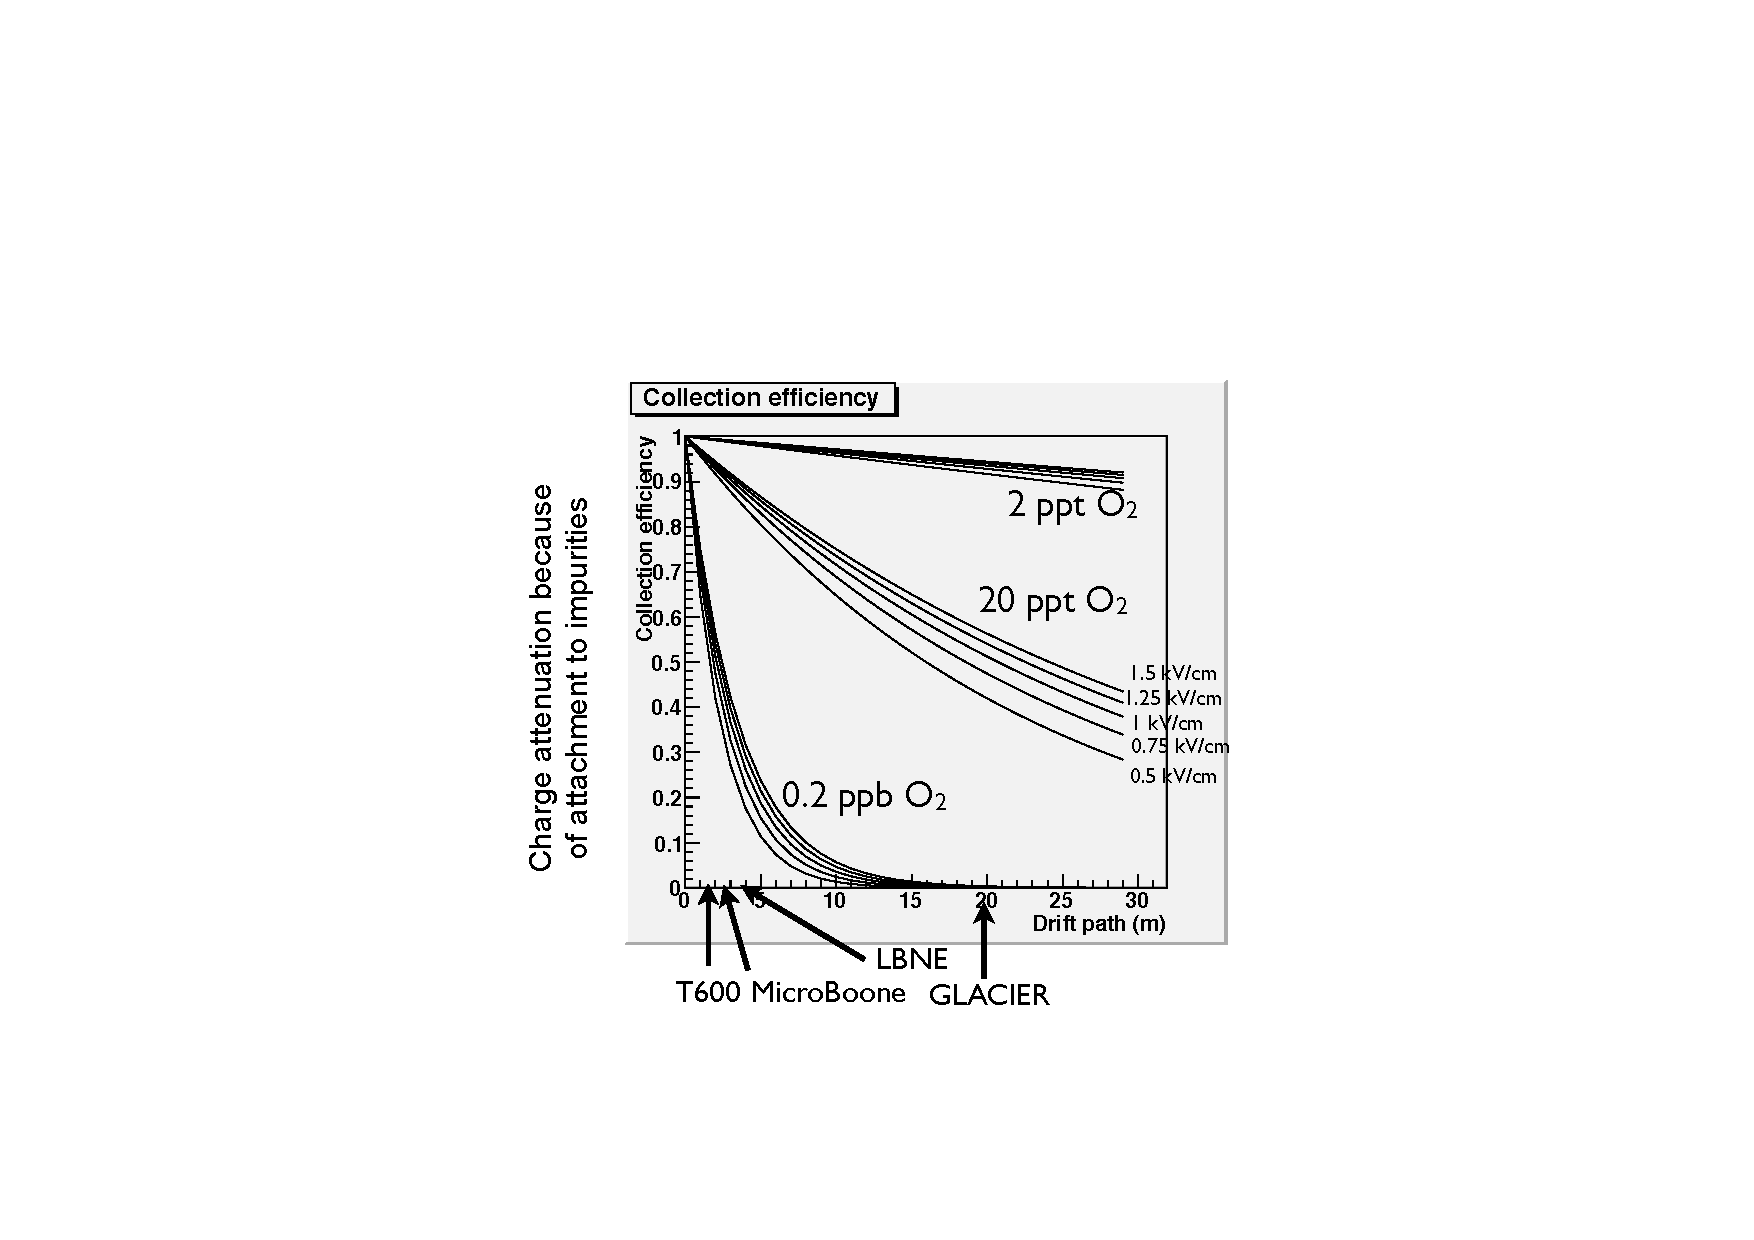
\includegraphics[width=0.6\linewidth]{Rubbia_Andre_fig2.pdf}
\end{cdrfigure}

The  free electro-negative molecules (like $O_2$, $H_2O$, etc.) must reach a level below 100~ppt $O_2$ level. An impurity level 
of $<30$~ppt $O_2$-equivalent is needed to obtain an electron lifetime greater than 10~ms. Compared to commercially available bulk liquid argon deliveries which typically contain ppm-level purities, the goal is to reduce those impurities by a factor $10^4$--$10^5$ before filling the main vessel tank. 

Excellent purity has been reproducibly achieved in various setups always relying on commercially available techniques, of various sizes and capacities, and should not pose a  show-stopper for long drift paths.

Several independent groups performed numerical simulations and experimental tests and  concluded that the vacuum evacuation of the main detector volume can be avoided for larger detectors, thanks to 
\begin{enumerate}
\item{ a more favourable surface / volume ratio for larger volume 
(also larger volumes are less sensitive to micro-leaks)}
\item{ a purification from ppm to $<<$ 1 ppb is anyhow needed
since the initial purity of argon when delivered is typ. ppm $O_2$ (see above)}
\item{  the outgassing of material is mostly from hot components
and impurities "frozen" at low temperature.}
\end{enumerate}

GAr flushing and purging were shown to be effective ways to remove air and impurities. Purging on 6~m$^3$ volume has been successfully demonstrated~\cite{Curioni:2010gd}. The piston effect was seen in gas and the impurities reached 3~ppm $O_2$ after several volumes exchange.

Although the double phase TPC adopts a drift length which is significantly longer than the others such as ICARUS T600, MicroBOONE or LBNE as mentioned above, it should be noted that all experiments require in order to collect efficiently ionisation charges a liquid argon purity
in the range below 0.1~ppb = 100~ppt of oxygen equivalent (Figure~\ref{Fig:larimpuritycomp}).  Hence, the challenge to reach the required level of purity starting from commercially available ppm-level bulk argon and a vessel which cannot be evacuated  is not mitigated by a shorter drift length in the meter range. It exists for all considered detectors.

\subsection{ DUNE double-phase LAr detector configuration.}

The proposed detector module, based on the double-phase design, optimally exploits the inner space foreseen for the DUNE cryostats ($14 (w) \times 14.1 (h) \times 62  (l) m^3$) with an active area of  ($12 \times 60 m^2$) and a drift length of 13 m corresponding to 13 kton of LAr. The proposed design is based on the one for 20 kton LAr detector of the LAGUNA-LBNO design study with a size of CRP unit in order to match in an optimal way the dimensions on the active area. The DUNE cryostat dimensions could be easily extended to host 15m of drift. In that case a single detector would reach an active mass of 15.12 kton.  Apart the shorter drift space with a shorter drift cage and the reduction of fiducial mass from 15.1 to 13 kton all the other detector characteristics, depending exclusively on the active area, are exactly the same for the the two detector configurations.

The detector is configured as LAr TPC with vertical, upward drift of the ionization electrons in the liquid phase, their extraction from liquid to vapor phase, via a horizontal extraction grid, towards a CRP (Charge Readout Plane). The CRP is composed by sandwiches of LEM (Large Electron Multiplier) for the charge amplification via avalanches occurring in a micro-pattern structure in pure gas argon and anode printed circuit boards (PCBs) for  the collection of the amplified charges on two independent orthogonal views with interleaved X and Y strips. Thicknesses and possible biasing voltages for the different layers are indicated, as example, in Figure~\ref{Fig:CRP_struct}). 

\begin{cdrfigure}[Charge Readout Plane (CRP) structure]{CRP_struct}{Thicknesses and HV values for e- extraction from LAr to GAr, their multiplication by LEMs and their collection on the X-Y CRP plane. The HV values are indicated for a drift field of 0.5 kV/cm in LAr.}
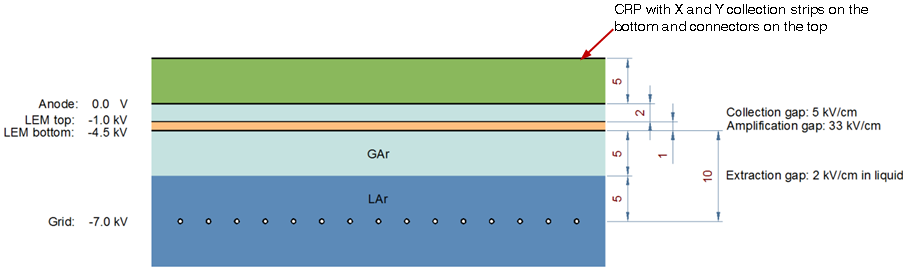
\includegraphics[width=\linewidth]{CRP_gaps.png}
\end{cdrfigure}

The inner detector for the 13 kTon active mass is built as a single active volume 60m long, 12m wide and 13m high. The active volume (see Figure~\ref{Fig:DP_det1} and Figure~\ref{Fig:DP_det2}) is surrounded by a vertical field cage made by a set of 75 rectangular tubular rings (tube diameter 140mm, vertical spacing 200mm).

\begin{cdrfigure}[Douple-phase detector 3D view]{DP_det1}{The DUNE double-phase detector with cathode, field cage, anode with chimneys and PMTs. X and Y coordinates are indicated, with Y along the direction of the LBL neutrino beam.}
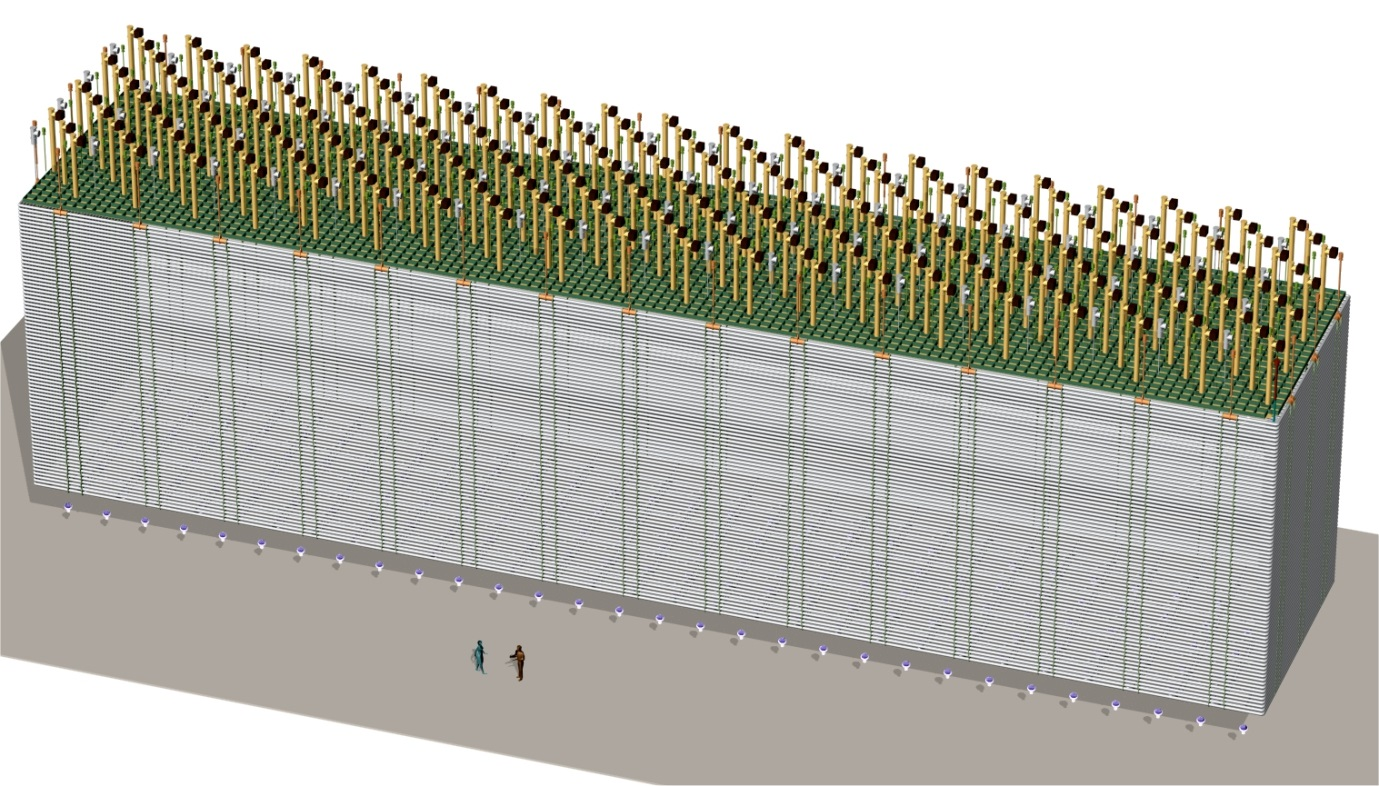
\includegraphics[width=\linewidth]{DP_det1.jpg}
\end{cdrfigure}

\begin{cdrfigure}[Douple-phase detector 3D view (partially open)]{CRP_struct}{The DUNE double-phase detector (partially open) with cathode, field cage, anode with chimneys and PMTs. X and Y coordinates are indicated, with Y along the direction of the LBL neutrino beam.}
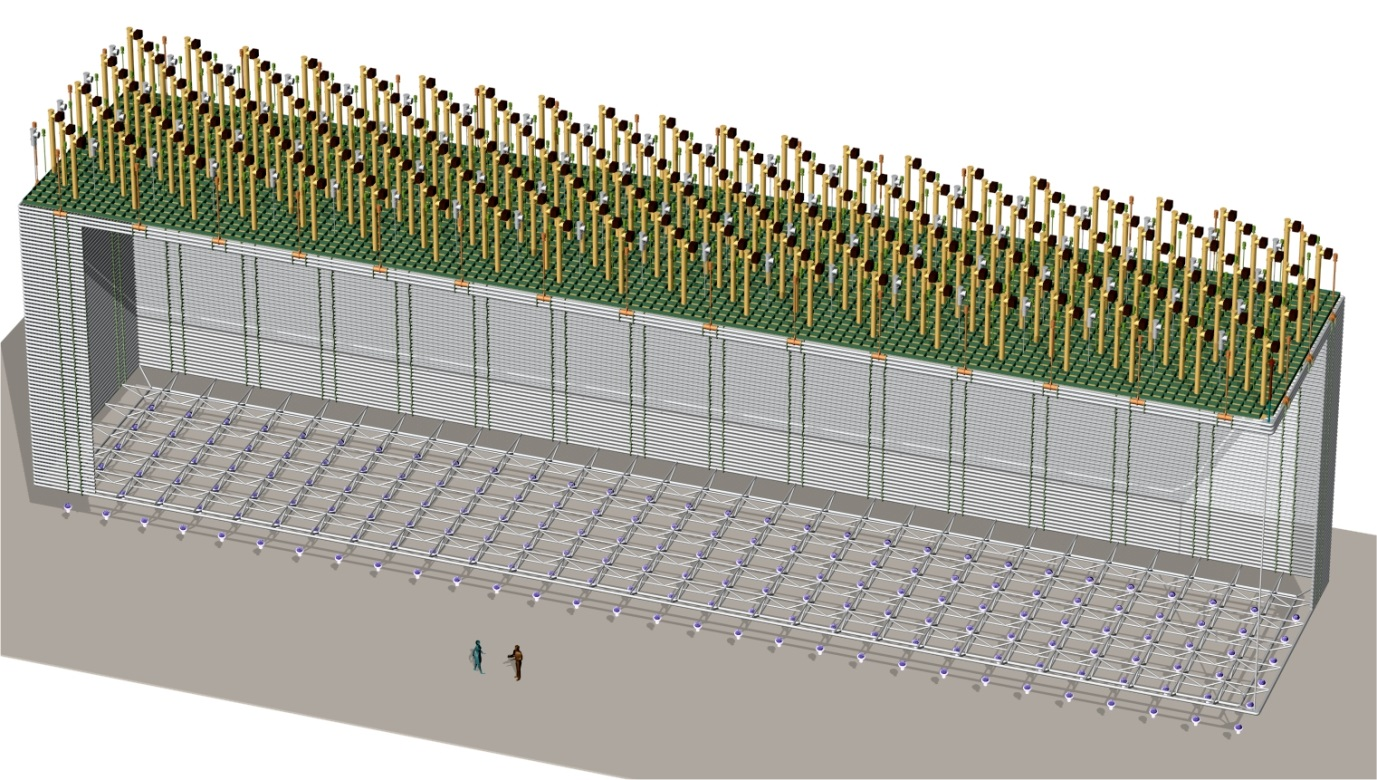
\includegraphics[width=\linewidth]{DP_det2.jpg}
\end{cdrfigure}

The cathode plane (on the bottom) is made by a reinforced frame, to guarantee its planarity, filled by a tubular grid (not visible in Figure~\ref{Fig:DP_det2}), to allow the optical transparency for the scintillation light toward an array of 180 PMTs (1 per 4m2) located at the bottom of the vessel.

The anode deck, at the top of the active volume, is made by an array of 45 indpendent CRP modules, $3\times3$ $m^2$ each, as shown in Figure~\ref{Fig:CRP_unit1} and Figure~\ref{Fig:CRP_unit2} Each CRP unit includes 36 LEM/Anode Sandwiches (LAS) ($0.5m\times 0.5m$) embedded in  a mechanically reinforced frame of FR-4 and Stainless Steel. 

Signals in each CRP unit are collected via 3 signal feedthrough chimneys. Each chimney collects 640 readout channels and hosts at its bottom the front-end cards with the cold electronics ASIC amplifiers, just before a second feedthrough isolating them from the ultra-pure LAr volume. The front-end cards work at a temperature of 110 K and can be removed from the top of the chimney without contaminating the LAr volume. The LEM/Anode sandiwiches in the same CRP unit are interconnected with short flat cables so that each readout channel corresponds to a total strips length of 3m.
  
Each CRP unit is independently suspended,  by 3 stainless steel ropes. The  vertical level of each CRP unit can then be automatically adjusted with respect to the LAr level via 3 suspension feedthroughs, electrically operated from outside. A Slow Control feedthrough + chimney, one per CRP unit, provides  information for level and temperature and provides HV bias for the two sides of the LEM  and for the extraction grid.

The extraction grid is made by an array X and Y oriented stainless steel wires, 0.1mm in diameter with 3.125mm pitch. 
Wires, ~12m long in X and ~60m long in Y directions, have sags minimized to ~0.1mm by supporting them by X and Y oriented suspending combs blades ( Figure~\ref{Fig:Wires_comb}) inserted between anode planes of $1m \times 1m$ size. The blade array, penetrating in the liquid, splits in sectors the LAr surface helping in maintaining it still.

\begin{cdrfigure}[DUNE CRP unit $3m\times 3m$).]{CRP_unit1}{ DUNE CRP unit $3m\times 3m$.}
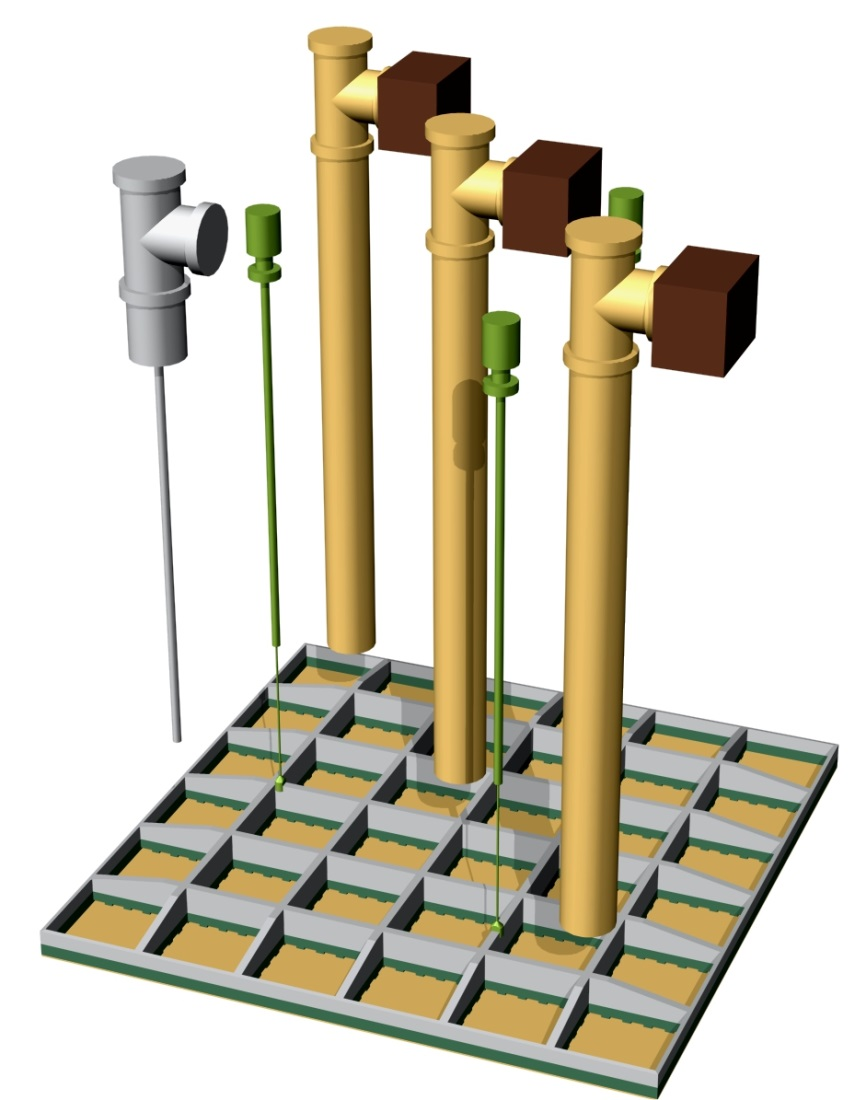
\includegraphics[width=.5\linewidth]{CRP_unit1.jpg}
\end{cdrfigure}

\begin{cdrfigure}[Signal collection in the X and Y views by the 3 SFT chimneys.]{CRP_unit2}{Signal collection in the X and Y views of the CRP unit by the 3 SFT chimneys.}
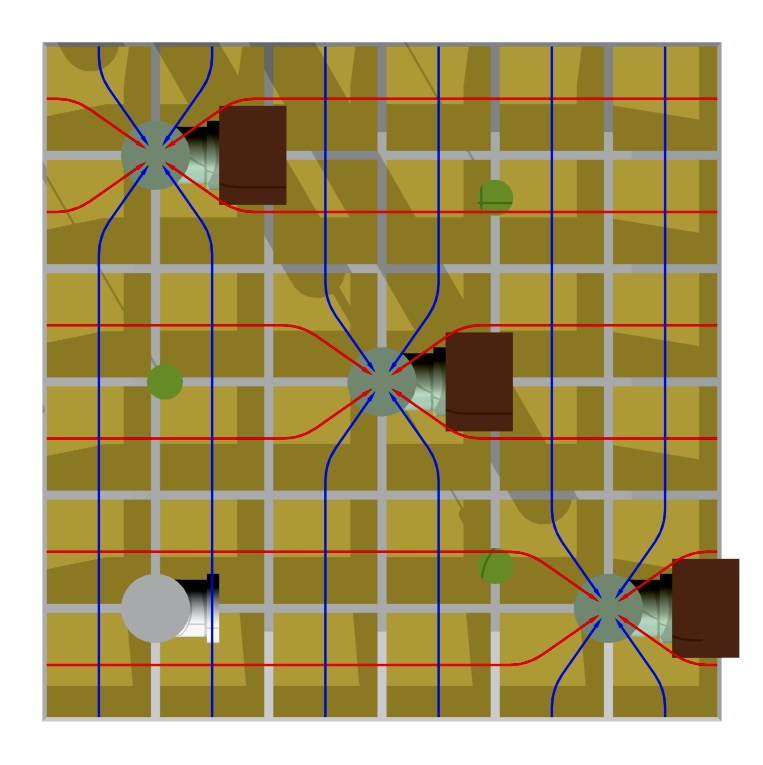
\includegraphics[width=.5\linewidth]{CRP_unit2.jpg}
\end{cdrfigure}

\begin{cdrfigure}[Wires hanging comb blade.]{Wires_comb}{Wires hanging comb blade.}
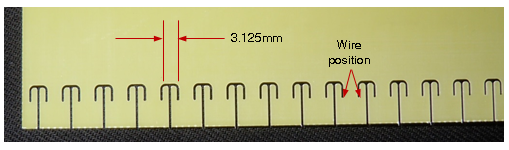
\includegraphics[width=.6\linewidth]{Wires_comb.png}
\end{cdrfigure}

The numbers of components and the parameters for the 13kT (15kT) double-phase  LAr TPC are summarized in Table~\ref{Tab:DP_params}.

\begin{cdrtable}[Components and parameters for the 13kT (15kT) double-phase LAr TPC]{clll}{DP_params}{Components and parameters for the 13kT (15kT) double-phase  LAr TPC}  
Item & & &  \\ \toprowrule
Active volume sizes & W = 12m &  L = 60m &   H = 15m (H=13m) \\ \colhline
Active volume / LAr mass & 10800 (9360) $m^3$ &  13104 (15120) Ton \\ \colhline
Number of field rings & 75  \\ \colhline
Field ring vertical spacing & 200 mm  \\ \colhline
Field ring tube diameter & 140mm \\ \colhline
Anode deck size & W = 12m & L = 60m \\ \colhline
CRP unit size & W =3m & L = 3m  \\ \colhline
Number of CRP units & 4 x 20 = 80 \\ \colhline
Number of LEM/Anode sadwiches per CRP unit & 36 \\ \colhline
Total number of LEM/Anode sandwiches & 2880 \\ \colhline
Number SFT chimneys /CRP unit & 3 \\ \colhline
Total number of SFT chimneys & 240 \\ \colhline
Number of read-out channels / SFT chimney & 640  \\ \colhline
Total number of read-out channels & 153600 \\ \colhline
Number of Suspension FT / CRP unit & 3  \\ \colhline
Total number of Suspension FTs & 240  \\ \colhline
Number of Slow Control FT / sub-anode & 1  \\ \colhline
Total number of Slow Control FTs & 80 \\ \colhline
Number of HV feedthrough & 1  \\ \colhline
HV for vertical drift & 600 - 900 kV \\ \colhline
Number of voltage degrader resistive chains & 4 \\ \colhline
Resistor value & 100 MOhm \\ \colhline
Total number of resistors & 300  \\ \colhline
Total number of PMTs & 180 (1 / 4 $m^2$) \\ 
\end{cdrtable}